\chapter{Stratégie de développement}
\newpage

\section{Méthologie de développement}
\subsection{Définition}

Ces derniers temps, un nouveau groupe de méthodes fait son apparition dans la
gestion de projet : on parle de méthodes agiles et Scrum fait partie de
celles-ci (voir figure~\ref{fig:scrum}). Le terme << agile >> définit une approche de gestion
de projet qui prend le contre-pied des approches traditionnelles prédictives et
séquentielles de type cycle en V ou waterfall.
La méthode dite « traditionnelle » favorise l’élaboration d’un plan détaillé
du besoin du client laissant donc peu de place au changement. Cela entraîne
souvent un effet tunnel, c’est-à-dire un manque de communication entre le
maître d’œuvre et le maître d’ouvrage, qui peut être néfaste pour mener à bien
le projet. Les membres du groupe de travail se rapportent alors aux
spécifications validées et au contrat. Certains projets se terminent dans la
douleur au risque de compromettre la relation client.
L’approche agile, elle au contraire, permet de réduire considérablement cet
effet tunnel en donnant davantage de visibilité. Pour cela, on implique le
client du début à la fin du projet et on adopte un processus itératif et
incrémental (processus qui implique l'intégration continue de l'architecture
d'un système pour produire des versions exécutables, chaque nouvelle version
contenant des améliorations incrémentales).
\\
\\

\begin{figure}[h]\label{fig:scrum}
  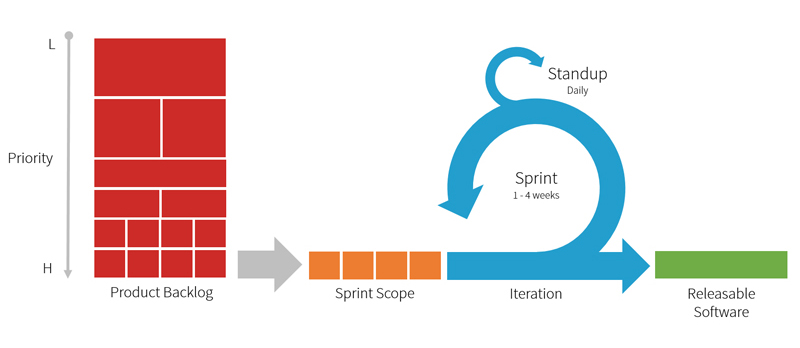
\includegraphics[width=\linewidth]{Scrum}
  \caption{schéma agile et scrum}
  \label{fig:scrum}
\end{figure}

\subsection{Application dans le projet lockatme}

Pour nous, utiliser une méthodologie agile, et plus particulièrement SCRUM s'est
traduit par une mise en place de sprint hébdomadaire à la fin desquelles nous nous
retrouvons pour fermer les tickets résolus et ouvrir de nouveaux tickets pour le
sprint d'après. De plus, nous essayons d'avoir de fréquents \emph{stand-ups}, des
petites réunion de 15 minutes généralement fait debout et qui permet d'exposer
d'une part les problèmes que l'on a dans l'avancé de notre travail et de se faire
aider et d'autre part, d'annoncer ce que nous comptons faire le jour même.

Les outils qui nous servent pour exploiter le potentiel de cette méthodologie est
\emph{Taiga} pour le suivit et la gestion des tickets et \emph{Discord} pour la
communication par message ou vidéo.

\section{Intégration continue}
Afin de collaborer au mieux au sein de l'équipe, nous avons mis en place
une C.I. (voir figure ~\ref{fig:CI-CD}). C'est un pipeline qui consiste à executer
les tests mis en places automatiquement après chaque changement sur une branche
du projet.
\vspace{0.5cm}

Après avoir positivement passé les tests et avoir subit une phase de review
pour recevoir commentaires et conseils, le code peut être intégré dans la
branche principale avec l'assurance (relative à l’exhaustivité des tests) qu'il
n'a pas compromis les autres parties du code.
\vspace{0.5cm}

Cette méthodologie de travail permet à l’utilisateur final de récuperer toutes
les nouveautés introduites au moment où elles sont \emph{merged} et non à la
sortie d’une nouvelle version. Dans certain cas, notamment avec les sites web
par exemple, on peut même arriver à faire du Continuous Deployment, ce qui veut
dire qu’il n’y a plus besoin de versionner les différents états du projet et
qu’à chaque push d’un des développeur, le site disponible à l’utilisateur est
celui contenant le dernier commit. Ceci n'est pas possible à faire pour un
projet comme le notre, qui doit être manuellement mis-à-jour à chaque nouvelle
version.

\begin{figure}[h]
  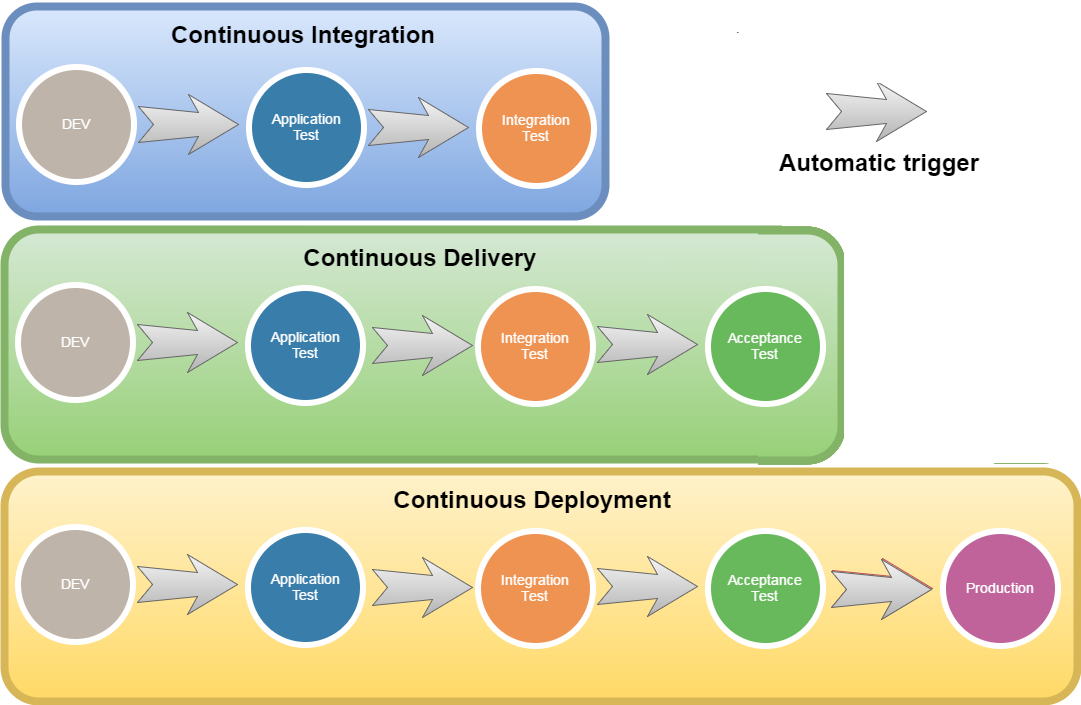
\includegraphics[width=\linewidth]{CI-CD}
  \caption{continious integration}
  \label{fig:CI-CD}
\end{figure}
